% ---------------------------------------------------------------------------
% Author guideline and sample document for EG publication using LaTeX2e input
% D.Fellner, v2, June 1, 2017

\documentclass{egpubl}

% --- for  Annual CONFERENCE
% \ConferenceSubmission % uncomment for Conference submission
% \ConferencePaper      % uncomment for (final) Conference Paper
% \STAR                 % uncomment for STAR contribution
% \Tutorial             % uncomment for Tutorial contribution
% \ShortPresentation    % uncomment for (final) Short Conference Presentation
%
% --- for  CGF Journal
\JournalSubmission    % uncomment for submission to Computer Graphics Forum
%  \JournalPaper         % uncomment for final version of Journal Paper (NOTE: this won't have page numbers)
%
% --- for  CGF Journal: special issue
% \SpecialIssueSubmission    % uncomment for submission to Computer Graphics Forum, special issue
% \SpecialIssuePaper         % uncomment for final version of Journal Paper, special issue
%
% --- for  EG Workshop Proceedings
% \WsSubmission    % uncomment for submission to EG Workshop
% \WsPaper         % uncomment for final version of EG Workshop contribution
%
 \electronicVersion % can be used both for the printed and electronic version

% !! *please* don't change anything above
% !! unless you REALLY know what you are doing
% ------------------------------------------------------------------------

% for including postscript figures
% mind: package option 'draft' will replace PS figure by a filname within a frame
\ifpdf \usepackage[pdftex]{graphicx} \pdfcompresslevel=9
\else \usepackage[dvips]{graphicx} \fi

\PrintedOrElectronic

% prepare for electronic version of your document
\usepackage{t1enc,dfadobe}

\usepackage{egweblnk}
\usepackage{cite}

% For backwards compatibility to old LaTeX type font selection.
% Uncomment if your document adheres to LaTeX2e recommendations.
% \let\rm=\rmfamily    \let\sf=\sffamily    \let\tt=\ttfamily
% \let\it=\itshape     \let\sl=\slshape     \let\sc=\scshape
% \let\bf=\bfseries

% end of prologue

% \input{EGauthorGuidelines-body.inc}

\title[Polygonal Model Compression]%
      {Polygonal Model Compression with Graph Symmetries}

% for anonymous conference submission please enter your SUBMISSION ID
% instead of the author's name (and leave the affiliation blank) !!
\author[Andrej Jočić]
{\parbox{\textwidth}{\centering% D.\,W. Fellner\thanks{Chairman Eurographics Publications Board}$^{1,2}$
        Andrej Jočić$^{1}$ 
%        S. Spencer$^2$\thanks{Chairman Siggraph Publications Board}
        }
        \\
% For Computer Graphics Forum: Please use the abbreviation of your first name.
{\parbox{\textwidth}{\centering %$^1$TU Darmstadt \& Fraunhofer IGD, Germany\\
         $^1$University of Ljubljana, Faculty of Computer and Information Science, Slovenia
%        $^2$ Another Department to illustrate the use in papers from authors
%             with different affiliations
       }
}
}
% ------------------------------------------------------------------------

% if the Editors-in-Chief have given you the data, you may uncomment
% the following five lines and insert it here
%
% \volume{36}   % the volume in which the issue will be published;
% \issue{1}     % the issue number of the publication
% \pStartPage{1}      % set starting page


%-------------------------------------------------------------------------
\begin{document}

% uncomment for using teaser
% \teaser{
%  
\includegraphics[width=\linewidth]{eg_new}
%  \centering
%   \caption{New EG Logo}
% \label{fig:teaser}
%}

\maketitle
%-------------------------------------------------------------------------
\begin{abstract}

We present a 3D mesh compression tool which compresses the connectivity information of polygonal models. The wireframe, treated as an undirected graph, is compressed with a graphlet dictionary approach. We also explore the use of automorphism-based compression, by which our algorithm is heavily inspired. We have implemented a proof-of-concept tool in Python, which can compress and decompress PLY files. Compression rates on some sample meshes show promise, but the tool is not yet practical for general use. We discuss the challenges of mesh reconstruction and the potential for future work. 

%-------------------------------------------------------------------------
%  ACM CCS 1998
%  (see http://www.acm.org/about/class/1998)
% \begin{classification} % according to http:http://www.acm.org/about/class/1998
% \CCScat{Computer Graphics}{I.3.3}{Picture/Image Generation}{Line and curve generation}
% \end{classification}
%-------------------------------------------------------------------------
%  ACM CCS 2012
%    (see http://www.acm.org/about/class/class/2012)
%The tool at \url{http://dl.acm.org/ccs.cfm} can be used to generate
\begin{CCSXML}
    <ccs2012>
    <concept>
    <concept_id>10010147.10010371.10010396.10010397</concept_id>
    <concept_desc>Computing methodologies~Mesh models</concept_desc>
    <concept_significance>500</concept_significance>
    </concept>
    <concept>
    <concept_id>10010147.10010371.10010387.10010394</concept_id>
    <concept_desc>Computing methodologies~Graphics file formats</concept_desc>
    <concept_significance>300</concept_significance>
    </concept>
    <concept>
    <concept_id>10003752.10003809.10010031.10002975</concept_id>
    <concept_desc>Theory of computation~Data compression</concept_desc>
    <concept_significance>100</concept_significance>
    </concept>
</ccs2012>
\end{CCSXML}

\ccsdesc[500]{Computing methodologies~Mesh models}
\ccsdesc[300]{Computing methodologies~Graphics file formats}
\ccsdesc[100]{Theory of computation~Data compression}


\printccsdesc   
\end{abstract}  
%-------------------------------------------------------------------------
\section{Introduction}

Polygonal models are widely used for representing 3D objects in computer graphics. With increased rendering system capabilities and the desire for greater precision, the size of these models has been increasing. To cut down transmission and static storage costs, specialized compression schemes have been developed.
In previously established \cite{meshCompressionSurvey} terms, we will be focusing on lossless single-rate global compression of static polygonal models. This means that we will be considering fixed (non-evolving) data, which will be decompressed it all at once (without progressive transmission at different levels of detail) and in its entirety (not focusing on specific regions of the model as requested by the user).

The information we usually store is the model's geometry (positions of vertices), connectivity/topology (incidence relations among elements), and optionally additional vertex/face attributes (normals, colours, etc.).
Typically, the connectivity information takes up the most space (around twice as much as the geometry information in a triangle mesh homeomorphic to a sphere \cite{rossignac1999edgebreaker}), so it is the most important to compress.
The vertex-to-vertex connectivity relations, also known as the \textit{wireframe} or the \textit{1-skeleton}
can be represented as an undirected graph.
This way we can reduce the mesh compression problem to that of graph compression.
One issue with this approach is that we lose face orientation data, which renderers need for shading and face culling. If a renderer can't infer consistent face orientations from the wireframe alone, we will need to encode this information separately. The issue is discussed further in section \ref{sec:reconstruction}.

Many compression methods focus exclusively on manifold triangle meshes (or another constrained structure) to get the best possible results.  
In this paper we will consider the case of arbitrary polygonal models, which may even be irregular (having faces of different degrees), although such models are not very common in practice. 
Specifically, we will be exploiting symmetries in the connectivity graph, which can often occur in the graphical domain.

\section{Mesh File Formats}

A typical mesh file format (e.g. OFF, PLY) has a header with metadata, followed by the vertex data, and finally the connectivity.
The topology is encoded as a list of faces, where each face is a list of vertex indices. Within a face we have one vertex index per edge, but usually the majority of edges are shared between two faces (assuming relatively few boundary edges). This means we have about 2 vertex indices per edge, which is a baseline for storing graphs. To do any better, we must encode the connectivity with less than 2 indices per edge, meaning we need to somehow compress the graph.

We decided to support compression and decompression of PLY files, since they are widely adopted and relatively simple in terms of structure.
Note that PLY has two formats: compact binary and human-readable ASCII. When reporting compression rates, we will be considering the binary format for a fair comparison with our (binary) compressed files.

Instead of the wireframe $W$ we could theoretically compress the \textit{face-to-face} 
adjacency graph, which is the \textit{dual} graph of the wireframe, $W^*$. Assuming $W$ is planar, we could get back $W$ at decompression by computing its dual again, since for planar $G$ we have $(G^*)^* = G$.
But this would just inflate the typical face-list mesh format, unless we could come up with more compact face descriptors than vertex lists.
If we are willing to give up the vertex-to-attribute mapping (and e.g. infer positions with a layout algorithm), we can just compress the connectivity information alone. In this case compressing the face incidence graph may be a viable option, since we don't have to list the vertices of each face but just an arbitrary face identifier.
% TODO discuss face rank encoding
However, this is not something we will be considering in this paper, since it does not seem like a common use case in the context of 3D graphics.

% \subsection{Related Work}
% slap some survey papers in here (graph compression, mesh compression)
% this and that paper has dealt with symmetry-based mesh compression, but to our knowledge it has not been done with automorphisms.

\section{Symmetry Compression}

Čibej and Mihelič \cite{cibej2021automorphisms} have developed a general graph compression method based on automorphisms (connectivity-preserving vertex permutations).
A graph $G$ is defined to be \textit{symmetry-compressible} (SC)
if it can be more succinctly represented with a ``residual'' graph $G^\pi$ and an automorphism  $\pi$ of $G$. Here $G^\pi$ is the minimal set of edges required to reconstruct $G$ by applying $\pi$ to its edges until all cycles of the permutation are closed.
Formally, $G \in \mathcal{S}\mathcal{C}$ if $\exists \pi \in Aut(G)$ such that $|G^\pi| + |\pi| < |G|$, where $Aut(G)$ is the group of $G$'s automorphisms and $|\cdot|$ denotes a measure of representation size (e.g. number of edges). 

The relative efficiency of a symmetry-compressed representation is defined as
$\Delta^r(\pi, G) = \frac{|G| - |\pi| - |G^\pi|}{|G|}$.
Note that for $G \in \mathcal{S}\mathcal{C}$, $\Delta^r(\pi, G) \in (0, 1)$ and higher values indicate better compression.


\subsection{Graphlet Search} \label{sec:graphlet}

The main computational issue in compressing a graph this way is finding a compressive automorphism $\pi$.
The problem is made somewhat easier by the fact that we only need to look for SC subgraphs. If we replace the subgraph's edges with their SC representation, we have reduced the representation size of the whole graph. 
Unfortunately the most common structure found in polygonal meshes, a triangle, is not SC \cite[Theorem 3]{cibej2021automorphisms}. Still, larger subgraphs of meshes may be SC, and looking for such graphlets is the approach presented in \cite[Algorithm 1]{cibej2021automorphisms}.

The procedure loops through a pre-computed list of SC graphlets with $n \leq n_{max}$, where $n_{max}$ determines the maximum size of the graphlets to be considered. 
For each graphlet $G^\prime$, it greedily extracts a maximal edge-disjoint set of subgraphs isomorphic to $G^\prime$, to be replaced by their SC representations.
As a heuristic, the graphlets are first sorted in decreasing order of relative efficiency to make sure that highly compressible ones are found before any of their edges have already been removed. We have opted to modify this algorithm, changing the compressed graphlet representation as described in the next section.

\section{Atlas-based Compression}

The algorithm described in the previous section very much resembles a dictionary-based compression scheme, although it is more generally applicable since it doesn't require an agreed-upon dictionary between the encoder and decoder. However, using large graphlets results in prohibitively long compression times, so we might as well make use of a small dictionary.
We have done this with the help of a \textit{graph atlas} \cite{read1998atlas}, a systematic enumeration of all undirected graphs up to a certain number of nodes $n$. Python's \texttt{networkx} library, which we have chosen for most of our graph data processing, provides access to the 1253 graphlets with $n \leq 7$.

Instead of encoding a subgraph $H \cong G^\prime$ with $(\pi, H^\pi)$ as in \cite[Algorithm 1]{cibej2021automorphisms}, we simply store the atlas index of $G^\prime$ and a mapping between nodes of $H$ and $G^\prime$.
Since this takes only $1 + n$ integers to store, it is always at least as efficient as the SC representation since an encoding of $\pi$ alone requires at least $n$ integers.
Thus, there is no reason to combine the representations, using the atlas for some graphlets and symmetry compression for others.

This may be seen as a sort of \textit{instancing} on a sub-mesh level. Instancing is a common technique for reducing the description size of a scene with many repeated objects (e.g. foliage elements) by only storing one copy of the object's geometric representation and associating each instance with its own coordinate transformation. In our case, we're ``storing'' one copy of a graphlet in the atlas and associating each instance with a vertex mapping, analogous to a coordinate transformation.

We can analogously define the relative efficiency of an atlas-based representation as
$\delta^r(G) = 1 - \frac{1+n}{2m}$ for a graphlet $G$ on $n$ nodes with $m$ edges. This can be used for sorting the graphlets in the same way as mentioned in section \ref{sec:graphlet}.
Note that the celebrated triangle, which is not SC, has $\delta^r(K_3) > 0$.
While all other connected graphlets with $n \leq 3$ are not atlas-compressible, it turns out that all connected graphlets with $n \geq 4$ are.

\textit{Proof:}
We must show $\frac{1 + n}{2m} < 1$ for $n \geq 4$. For a connected graph we have $m \geq n - 1$, so $\frac{1 + n}{2m} \leq \frac{m + 2}{2m} < \frac{m + 3}{m + m} \leq 1$ since $m \geq n - 1 \geq 3$ for $n \geq 4$.

\subsection{Compressed file format}

Our first approach to serializing the atlas-compressed mesh to binary was as follows. The header and vertex data are simply copied from the original PLY into their own file.
The atlas-compressed connectivity data is written to another file as a series of 4-byte unsigned integers:
\begin{enumerate}
        \item number of edges
        \item each edge, as a pair of vertex indices
        \item number of compressed subgraphs
        \item for each subgraph: its atlas index, followed by $n$ vertex indices (the node mapping).
\end{enumerate}
Note that we can infer $n$ (the size of the graphlet) from the atlas index, so we don't need to store it explicitly. But this approach may duplicate the same atlas index many times, if graphlets often reoccur in the mesh. Indeed, we have observed very skewed distributions of graphlet frequencies in the meshes we tested (see Fig. \ref{fig:graphlet_freqs}).
\begin{figure}[htb]
\centering
% the following command controls the width of the embedded PS file
% (relative to the width of the current column)
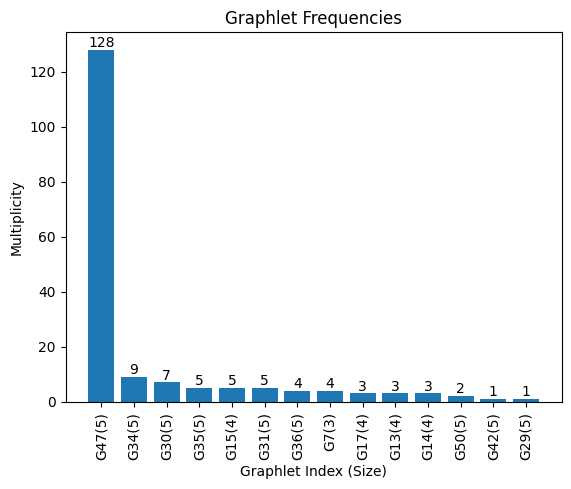
\includegraphics[width=.8\linewidth]{figures/nonmf_hole_freqs.png}
% replacing the above command with the one below will explicitly set
% the bounding box of the PS figure to the rectangle (xl,yl),(xh,yh).
% It will also prevent LaTeX from reading the PS file to determine
% the bounding box (i.e., it will speed up the compilation process)
% 
\includegraphics[width=.95\linewidth, bb=39 696 126 756]{sampleFig}
%

\caption{Graphlet frequencies in \texttt{non\_manif\_hole.ply} (Table \ref{tab:compression_nonmanif}) with $n_{max} = 5$.}
\label{fig:graphlet_freqs}
\end{figure}

So we also implemented an index multiplicity encoding, which stores (1-3) same as above, but then for each \textit{unique} atlas index, we store the index and the number of times it occurs in the mesh, followed by this many vertex mappings. This yielded notable increase in relative efficiency. % TODO show some data on this

In theory this encoding is only better if the total number of compressed graphlets is more than twice the number of unique atlas indices; in other words, if the average multiplicity of each atlas index is more than 2. For our application this is pretty much always the case, so we use this encoding unconditionally. Otherwise, we could have used a hybrid approach, where we fall back to the first encoding if the average index multiplicity is too low. This just requires an extra bit in the compressed binary to signal how it should be decoded.

\subsection{Experiments}

We have tested our implementation on some of the sample meshes provided with MeshLab. They can be downloaded here: \httpAddr{meshlab.net/\#download}.
Table \ref{tab:compression_nonmanif} shows compression performance on \texttt{non\_manif\_hole.ply}, a non-manifold mesh with 755 triangles.
\begin{table}
        \centering
        \begin{tabular}{|c|c|c|c|c|}
        \hline
        $n_{max}$ & $\delta^r(W)$ & $R_{conn}$ & $R_{total}$ & time \\
        \hline
        4 & 0.534 & 45.0\% & 64.2\% & 0.4s \\
        5 & 0.564 & 42.1\% & 62.3\% & 2s \\
        6 & 0.596 & 39.0\% & 60.3\% & 17s \\
        7 & 0.633 & 35.4\% & 57.9\% & 3min 5s \\
        \hline
\end{tabular}
\caption{Compression performance on \texttt{non\_manif\_hole.ply} with different $n_{max}$ (maximum graphlet size). Relative efficiency $\delta^r$ is computed over the whole wireframe, $R_{conn}$ is the compressed-to-original size ratio for the connectivity data, $R_{total}$ is the ratio for the entire PLY file.}
\label{tab:compression_nonmanif}
\end{table}
The reported compression time is achieved on a Ryzen 7 5800X3D machine with 32 GB of RAM,
with a pure Python implementation.
Evidently having graphlets with sizes up to 7 is good enough, because we are already approaching the limits of practicality.

We also tried simply zipping the PLY file. This yielded a very similar compression rate, which reflects poorly on the efficiency of our serialization. However, the general-purpose file compressor is also allowed to zip the vertex data, which we have left untouched. Of course, we can still zip our binary output to exceed the performance of the general-purpose compressor.

% TODO?: list connectivity comp. rates from survey table 1
% Typically, mesh compression rates are reported in bits per vertex (bpv) or bits per triangle (bpt). We will be reporting our results in bits per edge (bpe), since this is the most relevant measure for graph compression.

Table \ref{tab:more_meshes} shows compression performance on other MeshLab sample meshes.
We have only shown the relative efficiency, since this is really the metric that tells us how appropriate this compression paradigm is for the graphical domain. Raw compression ratios would be more informative given a more bit-efficient encoding and combination with vertex data compression, which we have not implemented.

\begin{table}
        \centering
        \begin{tabular}{|c|c|c|c|c|}
        \hline
        name & triangles & $\delta^r(W)$ & time \\
        \hline
        bunny2 & 1000 & 0.522 & 0.5s \\
        bunny10k & 9999 & 0.531 & 4s \\
        bunny70k & 69451 & 0.537 & 31s \\
        screwdriver & 13574 & 0.534 & 7s \\
        \hline
\end{tabular}
\caption{Compression performance on more sample meshes with $n_{max} = 4$.}
\label{tab:more_meshes}
\end{table}



\section{Near-Symmetry Compression} \label{sec:near_symmetry}

We have also explored the second algorithm presented in \cite{cibej2021automorphisms}, which is based on finding \textit{near symmetry-compressible} (NSC) subgraphs.
These are graphs that become SC if we add and/or remove a relatively small number of edges.
Formally, $G \in \mathcal{N}\mathcal{S}\mathcal{C}$ if $\exists H, \pi \in Aut(H)$ such that $|H^\pi| + |\pi| + |H \oplus G| < |G|$. Note that $\mathcal{S}\mathcal{C} \subset \mathcal{N}\mathcal{S}\mathcal{C}$.
The relative compression efficiency for a NSC graph is defined analogously to the SC case.

To compress a graph using this representation,
we must find a (small enough) edge difference $H \oplus G$ that makes computing $\pi$ easier.
Again we only need to look for NSC subgraphs, since
if $H \subseteq G$ and $H \in \mathcal{N}\mathcal{S}\mathcal{C}$, then $G \in \mathcal{N}\mathcal{S}\mathcal{C}$. This is the approach presented in \cite[Algorithm 2]{cibej2021automorphisms}, described in the next section.

\subsection{Bipartite Subgraph Completion} \label{sec:bipartite}

The idea is to repeatedly find near-complete bipartite subgraphs of $G$ (which have high relative efficiency) and replace them with their NSC representation. These are found by a greedy optimization starting from each vertex of the graph.

To keep track of such subgraphs we used a priority queue, sorted by relative efficiency. When extracting a subgraph $G(U,V)$, we must invalidate all queue entries that share an edge with it. 
We implemented two caching modes: static and dynamic. In the static mode, we only invalidate cache entries. In the dynamic mode, we also recompute locally optimal bipartite subgraphs from each $x \in U \cup V$. We don't even have to check if they are better than the cached ones, since the cache is already sorted by relative efficiency and the better ones will be extracted first (invalidating the worse ones).

Even the dynamic caching mode (which runs significantly slower) yielded very poor relative efficiency
(around 0.1 - 0.15 for the meshes we tested), so we did not pursue this avenue further.

These results may be explained by the fact that typical polygonal meshes are planar or locally plane-like (they have Euler characteristic close to 2). A complete bipartite graph $K_{n,m}$ with $n \geq 3$ and $m \geq 3$ contains $K_{3,3}$ as a subgraph, so it isn't planar by Wagner's theorem.
This means the only complete bipartite graphs that may often appear in the graphical domain are $K_{1,n}$ (a star) and $K_{2,n}$, but the former
is not symmetry-compressible \cite[Theorem 2]{cibej2021automorphisms}. Indeed, $K_{1,n}$ is not even NSC (by \cite[Theorem 6]{cibej2021automorphisms}).
The vast majority of extracted subgraphs we observed for meshes was $K_{2,2}$, which does not have a very good relative efficiency $\Delta^r(K_{2,2}) = \frac{1}{8}$ (note that this value falls in the above-reported range of efficiencies).

Of course, we could theoretically also find a symmetric difference $G(U,V) \oplus K(U,V)$ to compress an incomplete bipartite subgraph $G(U,V)$, but evidently meshes are too sparse to make this difference small enough for $\Delta^r > 0$. % TODO: try to prove this is always the case for planar graphs?


\section{Mesh Reconstruction} \label{sec:reconstruction}

When it comes to reconstructing the original mesh,
decompressing the wireframe is hardly the end of the story.
To produce the list of faces, we need to compute the facial walks of the wireframe.
In the case of a regular mesh (with all faces having the same degree), we can just enumerate all simple cycles of this length. This has time complexity $O((f + n)(d - 1)k^d)$ for a graph with $n$ vertices, $f$ faces of degree $d$, and average vertex degree $k$. Even though $k < 6$ for planar graphs, this can still take quite a while for large meshes.
For the 10 thousand triangle bunny mesh listed in Table \ref{tab:more_meshes}, this took 3 entire minutes!

Otherwise, if we are enumerating cycles of varying degrees, we need to ensure that all faces of non-minimal degree are \textit{chordless}, i.e. they don't have any diagonals. This even further increases decompression time. % TODO figure out the time complexity of this
Note that our decompressor does not support such non-regular meshes, since they are not very common in practice.

There is also the issue of \textit{internal} cycles, whose corresponding faces would end up inside the mesh (just under the surface). % TODO show an example of this
We have made the safe assumption that the original mesh has no internal faces, so we can filter these out. They can be identified as the faces with all edges incident on more than two faces.

The facial walks also lack a crucial piece of information: face orientation. We can think of this as a clockwise or counter-clockwise vertex ordering (from a fixed perspective). This information is needed by renderers to compute the surface normals (for shading etc.) and to decide which faces are front-facing (for culling).
We tried opening decompressed meshes in Blender 4.0 and MeshLab 2023.12 without addressing this issue.
We have observed that Blender 4.0 can fix inconsistent face orientations automatically, but MeshLab did not attempt to do so, resulting in incorrect shading on about half of the faces (Fig. \ref{fig:t_disoriented}).
\begin{figure}[htb]
\centering
\includegraphics[width=.6\linewidth]{figures/t_disoriented.png}
\caption{Improperly oriented faces of \texttt{T.ply} from MeshLab's sample meshes, as displayed in the program. This is a quad mesh, for which we have not implemented a solution. The issue is not reproduced in Blender.}
\label{fig:t_disoriented}
\end{figure}
We have only implemented a solution for orientable triangle meshes, where we can arbitrarily fix the orientation of one face (on each connected component) and propagate it to the rest of the mesh. This could be easily extended to general orientable manifolds, but for any others it is unclear how to compute a reasonable orientation. In that case, we could just store the face orientation data separately as a bit-vector, but this requires a reproducible ordering of faces (e.g. rank in lexicographic ordering).
This is a worthwhile feature to pursue in the future, since it would allow us to carry over arbitrary face data (like colours) that can appear in PLY files; for now we have ignored such data. 
% TODO discuss the canonical face walk thing
But coming up with a reproducible ordering of faces comes with the issue of single-face holes (see Fig. \ref{fig:bunny_holes}).
Since these can't possibly be inferred from the wireframe alone, we would need to find them at compression time and store them separately.
This is such a niche case that we have simply ignored it in our implementation. This results in such holes being patched up in the decompressed mesh.
\begin{figure}
\centering
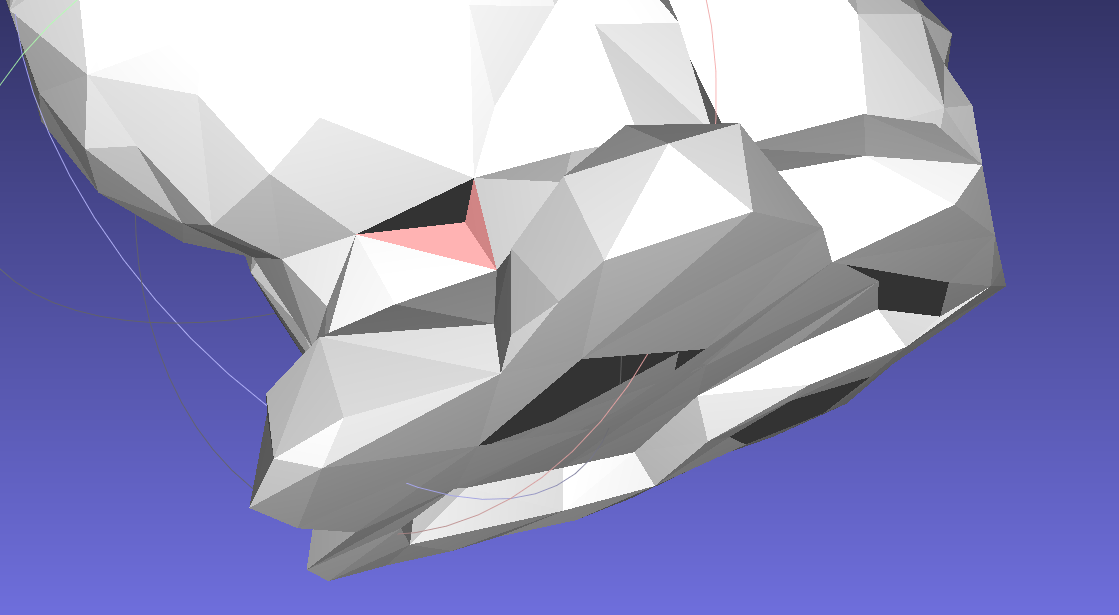
\includegraphics[width=.8\linewidth]{figures/bunny2_holes.png}
\caption{Holes at the base of the \texttt{bunny2.ply} mesh. The one consisting of a single triangle (above red-tinted triangles) can't be inferred from the wireframe alone. The larger ones (below) are kept in the reconstructed mesh since their boundaries are longer than 3, while the single-face hole is erroneously patched up.}
\label{fig:bunny_holes}
\end{figure}

\section{Conclusion}

We have implemented a proof-of-concept mesh compression tool,
available at \httpAddr{github.com/andrejjocic/mesh-compressor}.
The tool can compress the connectivity data in a PLY file to around 45\% of its original size, but many potential improvements remain.

\subsection{Future Work}

The class of near-symmetry compressible graphs discussed in section \ref{sec:near_symmetry} is a very general formulation, from which we could derive many domain-specific algorithms. The bipartite completion algorithm unfortunately turns out to be unsuited for the graphical domain, but we could come up with something more tailored to the structure of polygonal meshes. For example, if we limit ourselves to manifolds, or even further, to triangular or quadrangular ones, we may be able to find highly compressive symmetries.
Alternatively, we could use the assumption of a (near-)planar graph to speed up certain computations like facial walk enumeration, % NOTE: how??
and reduce the search space for automorphisms (e.g. filter out non-planar graphlets in a matching algorithm).
The heuristic sorting of graphlets could also account for common graphlet frequencies in the graphical domain, which we have observed to be very skewed. This way we might even break out of the loop over graphlets early (based on a relative efficiency threshold), allowing us to look for larger ones without running into prohibitively long compression times.

We have not done a very extensive evaluation of our compressor. Since the efficacy of this kind of compression is very much dependent on the density of the mesh, we would like to observe performance metrics \textit{with respect to} mesh density. To make these metrics comparable, we obviously don't want to use completely different meshes, but rather meshes of the same object with different levels of tessellation. 
A principled way to generate such a series from a point cloud $S$ is a \textit{filtration}, a construction from topological data analysis.
This is a sequence of \textit{simplicial complexes} (something very similar to a triangle mesh) obtained by varying a parameter $r$, where increasing $r$ increases the density of the complex in some way, as defined by the particular type of complex. Perhaps the most appropriate choice for the graphical domain is the \textit{Čech complex} Č$(S,r)$, which preserves many geometric properties of the point cloud.

We have limited ourselves to the simplest case of lossless single-rate global compression of static data. But the approaches we have described may naturally be extended to other compression modalities. For example, lossy compression could be achieved by replacing graphlets with ones that can be represented more compactly, but are not too different. In the graphical domain, we should formulate this notion of similarity based on human perception. Such perceptual metrics have been studied in the literature \cite{corsini2013perceptual}.


%-------------------------------------------------------------------------

%\bibliographystyle{eg-alpha}
\bibliographystyle{eg-alpha-doi}

\bibliography{references}

\end{document}
